%PAGINA 1


\begin{frame}
    \frametitle{Planteamiento del Problema}
    Los \emph{High Altitude Balloons} (HAB) son herramientas de bajo costo y eficaces para la exploración espacial inicial \cite{Saad2015}, ampliamente utilizados por instituciones educativas y agencias como la NASA \cite{noaa_radiosondes} y NOAA para obtener datos atmosféricos y realizar investigaciones científicas \cite{Jarrell2017}. Ver Fig. \ref{fig:globo} y \ref{fig:globo2}.

    \begin{figure}
        \centering
        \begin{minipage}{.5\textwidth}
            \centering
            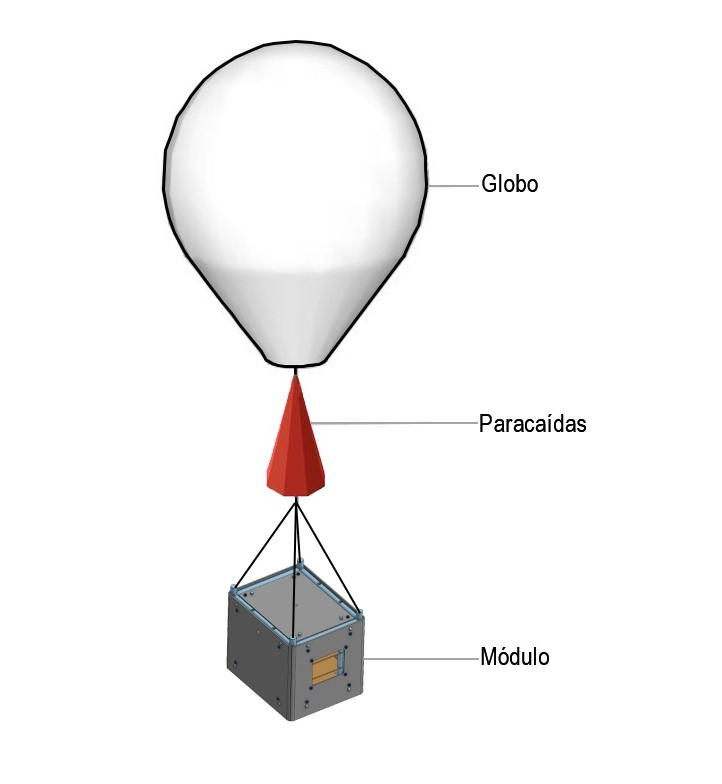
\includegraphics[width=0.38\textheight]{01_componentes del globo.jpeg} % Reemplaza con tu primera imagen
            \mycaption{Configuración de un HAB.}
            \label{fig:globo}
        \end{minipage}\hfill
        \begin{minipage}{.5\textwidth}
            \centering
            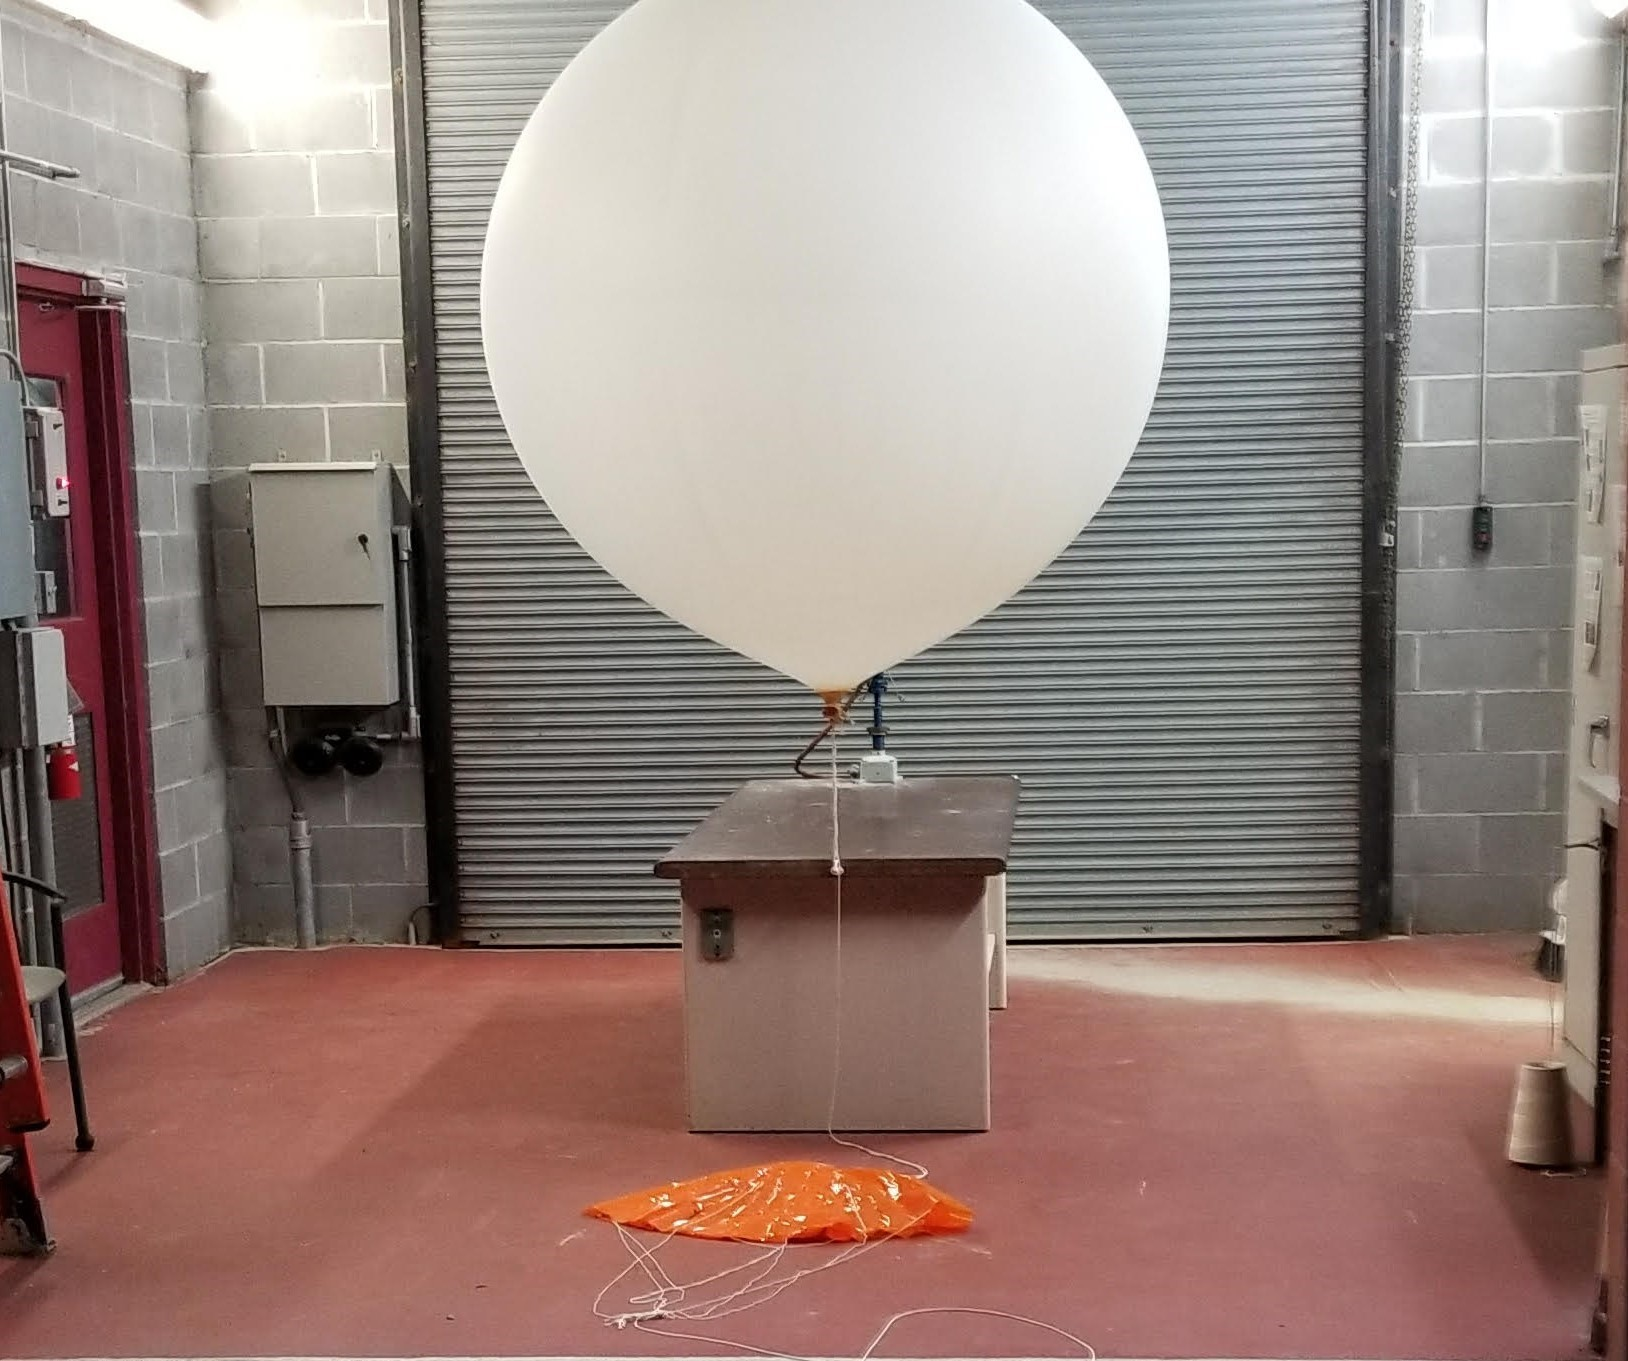
\includegraphics[width=0.45\textheight]{WeatherBalloon_NOAA.jpg} % Reemplaza con tu segunda imagen
            \mycaption{Globo meteorológico de NOAA \cite{noaa_upperair}}
            \label{fig:globo2}
        \end{minipage}
    \end{figure}
\end{frame}


%PAGINA 2


\begin{frame}
    \frametitle{Planteamiento del Problema}
   El proyecto StratoBalloon, una misión de HAB desarrollándose en el Observatorio Micro-Macro de la Universidad Don Bosco, requiere un sistema de energía eficiente y fiable para sus instrumentos (Fig. \ref{fig:electronica}). Este trabajo, enfocado en el diseño y simulación del sistema, propone soluciones basadas en software libre y componentes comerciales (\emph{Commercial Off-The-Shelf}, COTS).

    \begin{figure}[H]
        \centering
        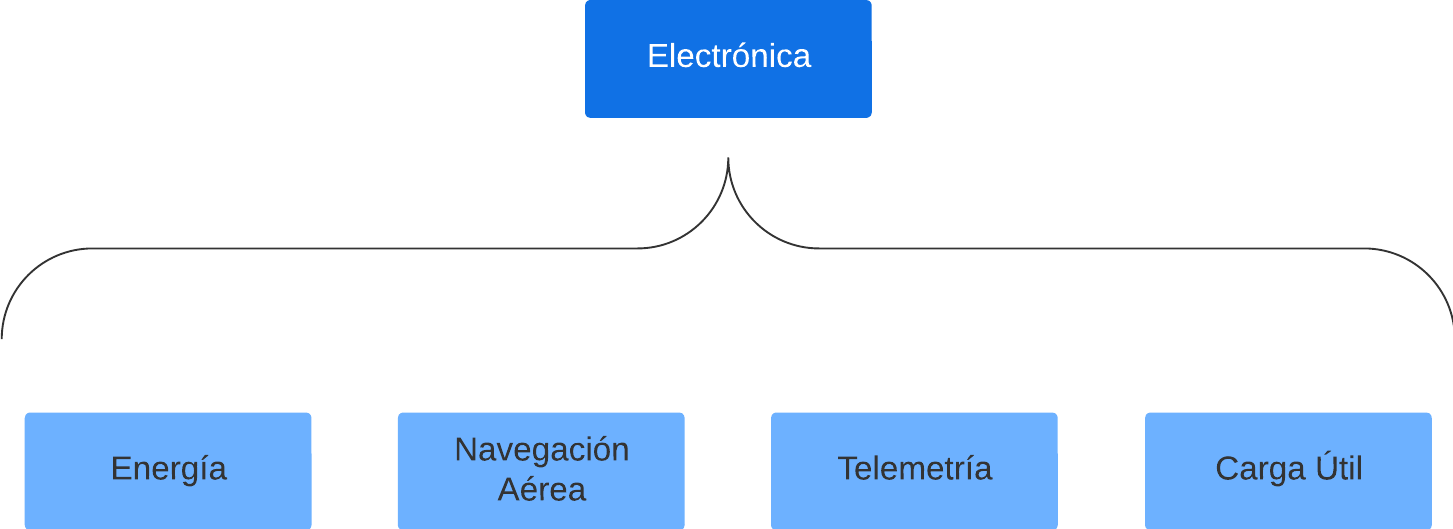
\includegraphics[width=0.75\textwidth]{Subsistemas.png} % Ajusta el tamaño según sea necesario
        \mycaption{Subsistemas electrónicos de misión StratoBalloon}
        \label{fig:electronica}
    \end{figure}
\end{frame}



% PAGINA 3

\begin{frame}
\frametitle{Objetivo General}

Diseñar un Sistema Eléctrico de Potencia (EPS, por sus siglas en inglés de \emph{Electrical Power System}) eficiente y confiable para misiones de corta duración en HABs, haciendo uso de componentes electrónicos COTS y software de código abierto.

\end{frame}

% PAGINA 4

\begin{frame}
    \frametitle{Objetivos Específicos}

\begin{itemize}
    \small
    \item Determinar las condiciones ambientales aproximadas que caracterizan las
    misiones de HAB a la estratósfera, a una altitud de 30 kilómetros.
    \item Establecer los requisitos eléctricos y energéticos necesarios para la misión,
    teniendo en cuenta los sistemas de navegación, telemetría y carga útil de la
    misión StratoBalloon.
    \item Diseñar tanto la arquitectura lógica como la física del EPS, con el propósito
    de identificar y seleccionar los componentes electrónicos y baterías más apropiados,
    considerando las condiciones de operación específicas de las misiones
    de HAB.
    \item Elaborar un plan de pruebas completo destinado a la verificación y validación
    del EPS de una sonda HAB, asegurando su correcto funcionamiento y
    confiabilidad en el entorno de la misión.
\end{itemize}

\end{frame}


% PAGINA 5
\begin{frame}
\frametitle{Metodología: Modelo V}
Este trabajo toma como Metodología el ciclo de proyectos de la NASA, concretamente 6 de las 7 fases, exceptuando la operación, ejemplificados en el Modelo en V (Fig. \ref{fig:ModeloV}).

\begin{figure}[H]
    \centering
    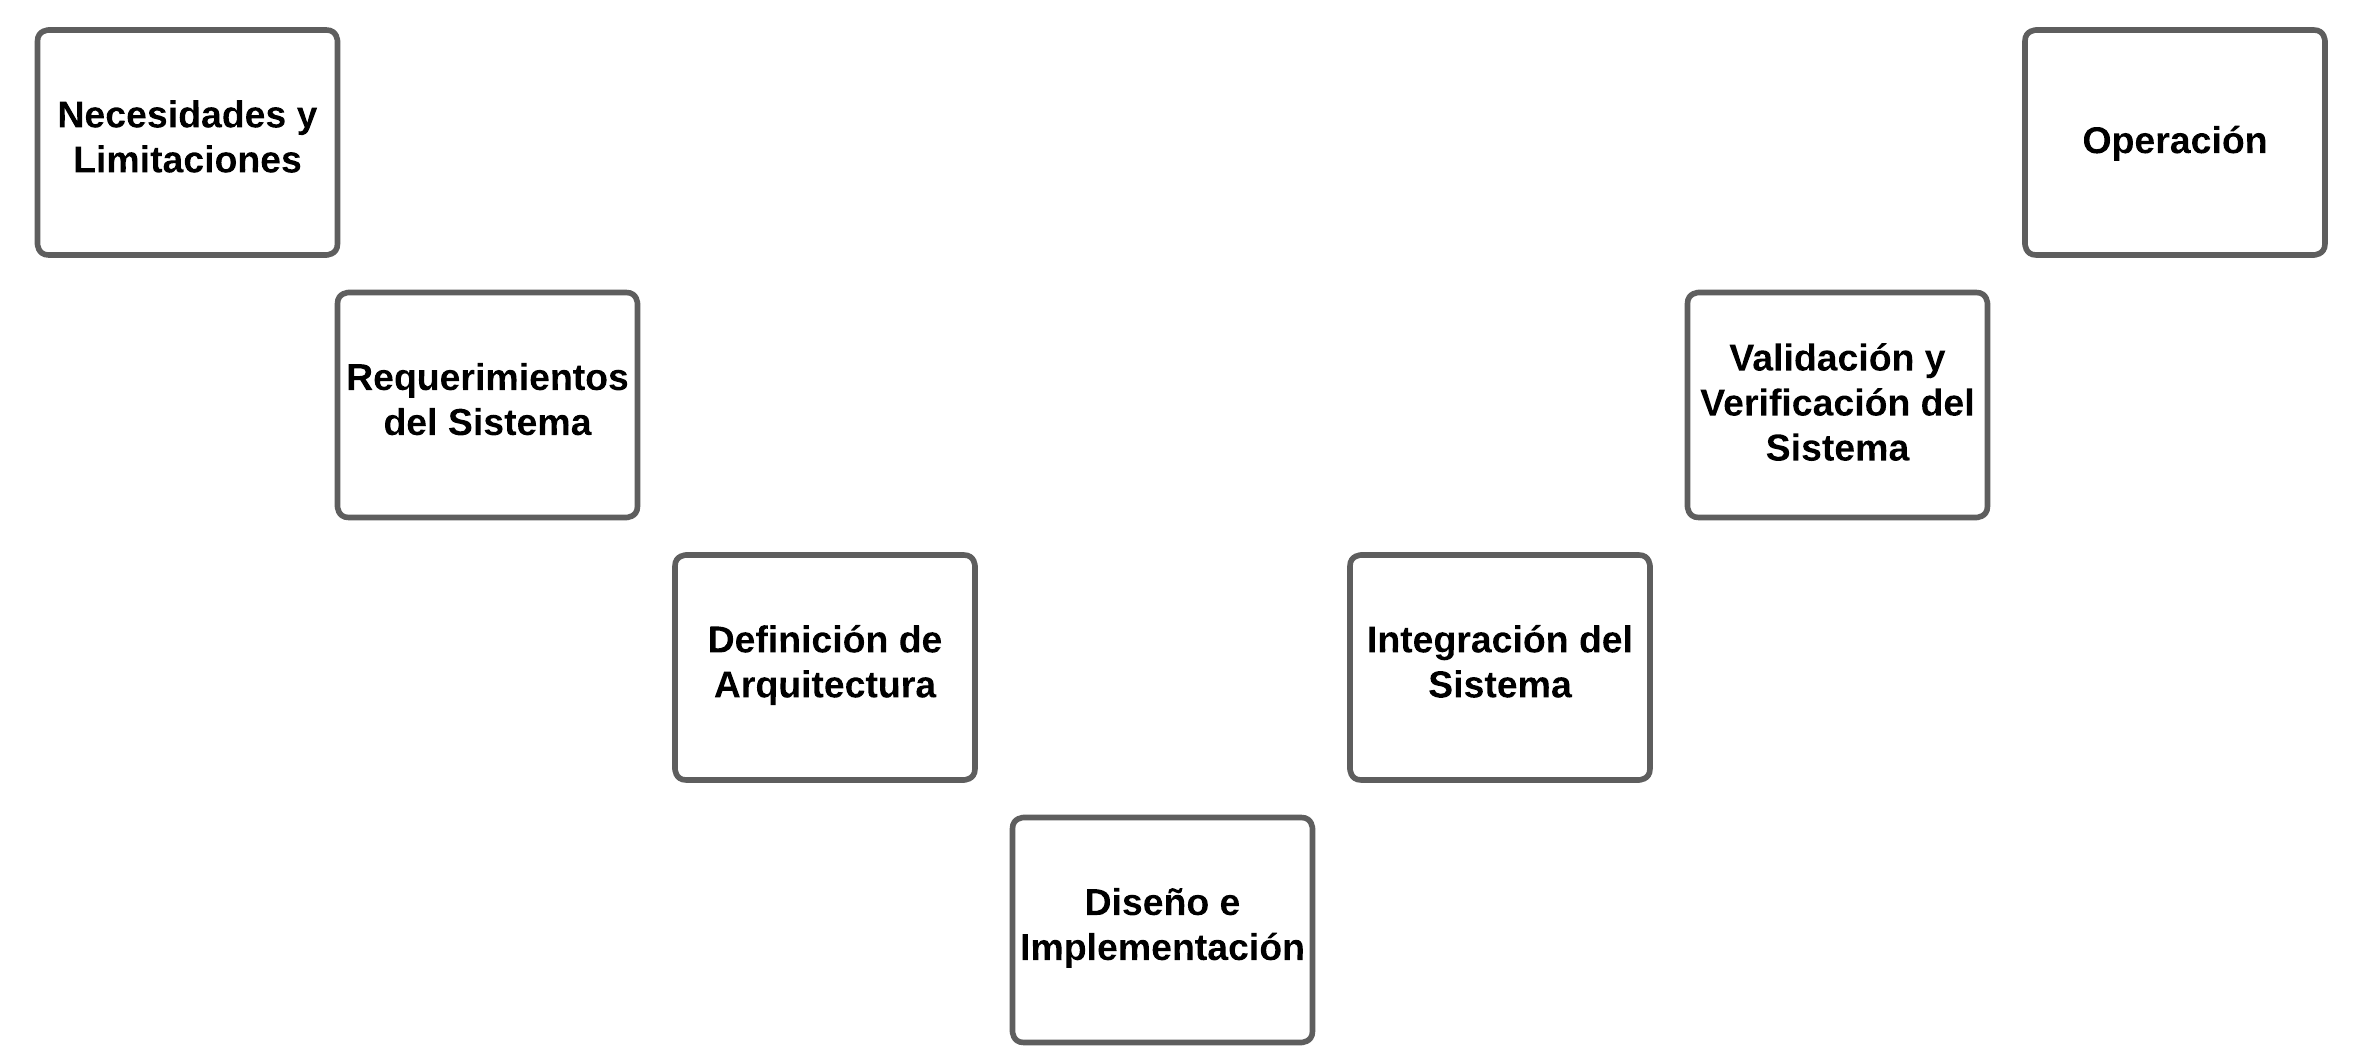
\includegraphics[width=0.9\textwidth]{modeloV.png} % Ajusta el tamaño según sea necesario
    \mycaption{Modelo en V basado en el NASA Systems Engineering Handbook \cite{NASA2016}.}
    \label{fig:ModeloV}
\end{figure}

\end{frame}

